% Sample file for AES paper
\documentclass{aes2e}

% Metadata Information
\jyear{2010}
\jmonth{October}
\jvol{1}
\jnum{1}


\begin{document}

% Page heads
\markboth{A1LASTNAME AND A2LASTNAME}{MIMIC in the OMOP Common Data Model}


% Title portion
\title{MIMIC in the OMOP Common Data Model\thanks{To whom correspondence should be addressed Tel: +1-240-381-2383; Fax: +1-202-508-3799; e-mail: info@schtm.org}}

%Author Info.
\authorgroup{
\author{A1FIRSTNAME A1LASTNAME},
\role{AES Member}
AND \author{A2FIRSTNAME A2LASTNAME},
\role{AES Fellow}
\email{(abc@abc.com)\quad\quad\quad\quad\quad\quad\quad\quad\quad\quad\quad\quad (xyz@abc.com)}
\affil{Universityxyz, City, Country}
}

%Abstract
\abstract{%
This paper discusses the implementation of spectral delay using
filters comprising a cascade of many low-order allpass filters and an
equalizing filter. The spectral delay filters have chirp-like impulse
responses causing a large, frequency-dependent delay that is useful in
audio effects processing. An equalizing filter design and a multirate
technique, which stretches the allpass filters, impulse
response, are introduced.}


\maketitle
%Head 1
\section{INTRODUCTION}
%
% 1. ICU and BIGDATA
% 2. MIMIC DB & its limitations
% 3. CDM can overcome this limitations (and are better than FHIR or I2B2 thanks to standard concepts)
% 4. OMOP is better
% 5. Evaluation method and importance of the work
%    Objective threefold are: 1. transform, 2. contribute 3. analysis
%
% ICU and BIGDATA
Intensive care units (ICUs) are care units where the demand for care 
increases\cite{angus2000} while mortality reaches up to 30\%, 
which is a major health problem\cite{icu-mortality}. 
Studies have shown that intensivists use a limited level of evidence 
to guide decision making\cite{icu-evidence} 
and that medical practices are sparse and variable.
Knowing that the ICU patient health record is very detailed and that there is 
a high density environment for data production is a paradox. 
The increasing adoption of electronic health record (EHR) systems 
around the world is capturing large amounts of clinical data\cite{bigdata-promise} 
and data mining has the potential to play an important role 
in clinical medicine\cite{bigdata-mining}. 
Indeed, based on important medical informations, expectations are 
to improve clinical outcomes and practices, 
enable personalized medicine and guide early warning systems, 
and also easily enroll a large, multi-center cohort while minimizing costs.

% MIMIC DB
% - local terminologies
% - one center
% - two successive critical care information systems (CCI)
% - a model that reflect the EHR
\emph{MIMIC} (Medical Information Mart for Intensive Care) 
is a 10 year semi-automatic dataset of over 60,000 intensive care stays 
with very high granularity (including EKG) 
from two successive intensive care information systems (CCI)
 at the Beth Israel Deaconess Medical Center in Boston. 
It is the first ICU database available free of charge and has been the subject 
of more than 300 international publications. 
However, its monocentric nature makes it difficult to generalize findings to other ICUs. 
The MIMIC relational data model reflects the original CCI, 
as evidenced by the two separate \textit{inputevent\_mv} and \textit{ouputevent\_cv} \cite{mimic-nature}
or the two separate terminologies for physiological data. 
This leads analysts (datascientists, statisticians, etc.) 
to reconcile this heterogeneity when pre-processing each study.

% Why a Common Data Models
Some studies have shown that using a common data model (CDM) by generalizing 
the structural (data model) and conceptual (terminological model) design database 
allows for multicentre research, exploitation of rare diseases 
and catalyzes research by sharing practices, source code and tools \cite{cdm-review,data-enclave}. 
As Kahn and Al said \cite(kahn-data-2012),  "databases modelling is the process 
of determining how data are to be stored in a database". 
It specifies data types, constraints, relationship and metadata definitions 
and provides a standardized way to represent resources/data and their relationships. 
However, some studies have shown that the results are not fully reproducible 
from one CDM to another \cite{cdm-comparison} or from one centre to another \cite{omop-replicability}. 
The lighter approaches argue that maintaining the local conceptual model \cite{fhir-deep}
or the original conceptual and structural model \cite{imi-protect} of the research database 
leads to better results. On the one hand, keeping MIMIC on its specific form 
will not solve the limitation for multicentric research and, on the other hand, 
a fully standardized form would introduce other disadvantages. 
The ideal solution is probably in between to allow 
local or standardized analysis depending on the research question.

% OMOP
\textit{OMOP} (Observational Medical Outcomes Partnership Common Data Model) 
is a CDM originally designed for multi-centre drug-related adverse events 
and now extends to medical, clinical and genomic cases. 
OMOP provides structural and conceptual models such as SNOMED for diagnostics, 
RxNORM for drugs and LOINC for laboratory results. Several examples of database 
transformation to OMOP have been published \cite{omop-german,omop-nashville} 
and OMOP stores 682 million patient records from around the world \cite{omop-bigboy}. 
Each clinical area is stored in different dedicated tables. 
The OMOP conceptual model is based on a closure table pattern \cite{closure-table} 
capable of ingesting any simple, hierarchical and also graph terminologies 
such as SNOMED-CT. In addition to local terminologies, OMOP specifies 
and maintains a set of standard terminologies to be mapped unidirectionally 
(local to standard) by implementers.
Although OMOP has proven its reliability \cite{omop-eval}, 
the concept mapping process is known to have an impact on results \cite{omop-concept-impact} 
and the application of the same protocol on different data sources 
leads to different results \cite{omop-replicability}. 
This shows the importance of keeping local codes so that local analysis is always possible.
Previous preliminary work has been done on the translation of MIMIC into OMOP \cite{mimic-omop-previous}. This work remains to be refined and updated to be evaluated.

% CDM Comparison
In a recent CDM comparative study \cite{cdm-review,omop-vs-pcornet}
OMOP obtained better results in the criteria of the evaluation database 
compared to the other models: completeness, integrity, flexibility, simplicity 
of integration and implementability, adapting to the wider coverage 
of standard terminologies, providing a more systematic analysis 
with an analytical library and visualization tools, providing SQL models easier to use.
That is why OMOP offers a broader set of standardised concepts.
In terms of structural CDM, OMOP is very rigorous in how data should be loaded 
into a particular table when i2b2 for example is very flexible 
with a general table that solves all data domains. This rigorous approach 
is necessary for standardization. 
Previous work has loaded i2b2 with MIMIC-III \cite{mimic-i2b2} - 
however, the concept mapping step has limited the results since i2b2 design 
does not store local ontologies or informations where OMOP design keeps 
concept mapping unfinished. OMOP has the advantage of not making the terminology 
mapping step mandatory by keeping local codes in a usable format. 
Compared to the FHIR, OMOP performs better as a conceptual CDM because 
the FHIR does not specify the terminology to be used. In terms of structural CDM, 
the OMOP relational model can be materialized in csv format
 and stored in any relational database when FHIR uses json files and 
needs some processing and more skills to exploit.
We believe OMOP shares the advantages of all the above models.

% Evaluation of MIMIC-OMOP
In order to evaluate the transformation of MIMIC into OMOP, 
we propose to answer the following questions, 
such as the difficulty of transforming/maintaining an OMOP dataset 
from an local database, how the initial data is integrated 
and how much data is lost in the process, how the model should be queried simply 
and efficiently by analysts, how the design should be enriched by collaborative work, 
and finally to what extent OMOP can integrate and feed back to intensivists 
in a real-time context. This work is then evaluated according to 3 axes: 
Transformations, Contributions and Analyses. 
% contribution
The \emph{first} major contribution of this study is to evaluate OMOP in a freely 
accessible and well known database. The \emph{second} major contribution is to provide 
a freely accessible dataset in OMOP format that could be useful to researchers. 
The \emph{third} major contribution is to provide the OMOP community with useful 
transformations dedicated to intensive care that can be reused on any OMOP data set.


\section{Material \& Method}
%\subsection{Data Transformation}

% ETL
The MIMIC-III version 1.4 21 (MIMIC) clinical data tables and 5 tables for vocabulary
OMOP CDM v5.3.1 (OMOP) which defines 15 standardized \textit{clinical} data tables, 3
\textit{health} system data tables, 2 \textit{health economics} data tables, 5 tables
for \textit{derived} elements and 12 tables for standardized
\textit{vocabulary}. The vast majority of the source code is implemented in
PostgreSQL 9.9 (PGSQL)
% We didn't use the health economics data tables (not provided by MIMIC)
All the process is publicly and freely available as a github website
\cite{mimic-omop-website} included and maintained by the MIT-LCP organization
responsive of the MIMIC maintenance and distribution \cite{mimic-nature}.  The
repository centralizes various resources of this work such documentation,
source code, unit tests, as well as query example, discussions and history of
issues. It also points to relevant resource such a website based physical data
model for both MIMIC and OMOP datasets and the Achilles webclient. The
repository is based on git and is designed for community sharing, improvement,
collaboration and reproducible work. Indeed github is archived on a universal
software archive solution \cite{universal-archive} and this implies its
sustainability.

Extract-Transformation-Load (ETL) processes is a methodology that allows
migrating data from a source location to a target location. ETL first extract
the data from the source location, and then apply transformations such
structural modifications or conceptual modifications generally on a dedicated
computer and technology. The last step is to load the resulting data into the
target location. Transformation program are generally written in a programming
language such java, c++ or python.
Extract-Load-Transform (ELT) processes is a slightly different methodology that
does not use a dedicated transformation server and limits data transfers. The
data is extracted and directly loaded into the target location. It is
transformed afterwards in place. ELT allows to factorize both computer
resources, and people knowledges. Indeed transformations are then written in a
database dialect such SQL, as well as source and target location. Improving
database resources will then benefit for both ETLers and end users. Since RDBMS
computer resources cannot scale well and does not provide a good support for
procedural language, ETL have been for long time used in conjunction with
RDBMS. The emergence of distributed platform such hadoop allows to take part
of ELT because they both allow to scale well horizontally and write java
procedural user defined function that are used in conjunction with SQL queries.
In this work, we decided to transform MIMIC into OMOP thought a ELT to limit
the programming knowledges needed for code maintenance and to allow end users
to participate in this process. PGSQL has been chosen as the database
support for ELT because it is the primary support of MIMIC database and allows
community to run the ETL on limited resources without licensing need. Finally
PGSQL have recently made huge effort to handle data-processing better.

% Structural Transformations

% creating tables (only with constraints, no indexes, subset, sequences)
% <!--Ajouter les deux schemas de database design -->
The MIMIC source data have been loaded with the provided scripts into a PGSQL
instance and a subset of 100 patient chosen upon their broad representativity
in terms of data have been cloned into a second instance to serve as a light,
representative development set.  Each tables of the source have been added a
global sequence incremented from 0 that serves as primary key and link into the
OMOP target tables. The target tables have been created from the provided
script except the indexes that would have slow down the data migration with
useless computations. The integrity constraints (primary keys, foreign keys,
non nullable columns) have been included to apply sanity checks at runtime.
Some tricky transformations have been implemented as PGsql functions.
The ETL is composed of 22 PGSQL scripts, each extracting information from the
source or from concept mapping tables, transforming and loading one OMOP target
table. The ordering of those scripts matters and is done sequentially thought a
main script.
% unit testing
Each ETL part have been tested thought pgTAP, a unit testing framework for PGSQL.
This allows to make sure there is no loss of informations, or code regression
during the ETL development or for further updates of the source code.
The unit tests are composed of 15 scripts, each checking a particular OMOP
target table is loaded correctly - most of the tables are covered and tests
covers simple counts, aggregated counts or distribution checks.
% DDL modification
A SQL script updates the OMOP tables when needed (the list of the modifications
is detailed bellow). 
All character typed columns limited in length have been changed to unlimited
since this might cause unpredictable truncation of content, and this has no bad
impact on PGSQL's storing size or performance.
The \textit{visit\_occurrence} and \textit{visit\_detail} table have been corrected
accordingly to some discussion on the forum.
The \textit{note\_nlp} table have been extended with some fields accordingly to
the documentation online. The character \textit{offset} column have been split into
two integers columns because the offset word is a SQL reserved word and it
makes sense to fill the resulting \textit{offset\_begin} and \textit{offset\_end}
resulting columns.

The structural transformation have been done in few iteration of several
phases. The first phase consists of looping over each MIMIC table and choose
for each columns an equivalent location in OMOP. In general, the MIMIC
documentation and the OMOP documentation were sufficient informative. In
several cases, we needed to get clarification from the MIMIC contributors on
the dedicated github repository, or from the OMOP community on the dedicated
forum.  All choices have been discussed in the repository issues
\cite{mimic-omop-github}, and can be tracked into the commit log. The resulting
table to table work flow is materialized in the repository as bi-directional
documentation: from MIMIC table to OMOP table and vice-versa.


% Preprocessing and modification of mimic
By design MIMIC aggregates informations from various systems such the emergency
specific tool. Thus the transfer information is spread into multiple table,
such \textit{admissions}, \textit{transfers} and \textit{icustays}. OMOP
centralizes this information in the \textit{visit\_detail}. As a result some
hard transformation have been made. We added emergency stays as a normal
location for patients throughout their hospital stay. Icustays mimic table was
deleted as it is a derived table from transfers table (2) and we decided to
assign a new new \textit{visit\_detail} pour each stay in ICU (based of the
transfers table) whereas mimic preferred to assign new icustay stay if a new
admissions occurs > 24h after the end of the previous stay.


% INUTILE? visit\_detail : admitting\_source\_value, admitting\_source\_concept\_id, admitting\_concept\_id, discharge\_to\_source\_value, discharge\_to\_source\_concept\_id, discharge\_to\_concept\_id provide redundant information from visit\_occurrence. We didn't populate it.
% INUTILE? observation\_period provide duplicate informations with visit\_occurrence : we fill this table to respect the OMOP model and toolsii

% Conceptual Transformations

% conceptual (new concepts specific to ICU or general)
While various types of information are stored in the measurement table, the
dedicated OMOP concepts types were not enough to distinct them. We added some
measurement types.
The actual visit\_detail doesn't introduce pertinent information and duplicate
informations from visit\_occurrence table. For admitting\_concept\_id and
discharge\_to\_concept\_id, we extended the dictionary in order to track bed
transfers and ward transfers. For visit\_type\_concept\_id we assigned a new
concept for any level of granularity necessary for your use case (ward, bed...) 
%<!-- Fournir un example de visit\_detail-->


% local coding
The conceptual transformation consists on both loading OMOP with the MIMIC
local concepts, and mapping them to the standards concepts. 
The local codes have been loaded in the concept table starting from 2 billion
as specified in the OMOP documentation \cite{omop-documentation-pdf}. The
MIMIC local codes are then added to the OMOP provided code (starting from 1 to
2 billion) and can be distinguished with the domain\_id equals to MIMIC code. As
much as possible information from the MIMIC coding table have been loaded in
order to allow analytics with the local code without loosing information as
compared to the MIMIC original model (worst case we concatenated information as
free text in the concept\_name column).
%concept mapping
To deal with concept mapping for each domain a csv file have been built as a
support for manual standard mapping. This solution can scale for medical users
without database engineering background. We tried to adopt the same methodology
in their creation ; some obvious fields are needed : local and standard name,
local and standard id. Moreover evaluation and comments fields are good
practices and may help contributers Those csv file are automatically loaded
into PGSQL and get the sequence added too. There were four distinct cases.  In the
\emph{first} case MIMIC is already in the OMOP standard terminology (eg: LOINC
laboratory results), the work is already made.  In the \emph{second} case the
mapping is already provided by OMOP (eg: ICD9/SNOMED-CT) then the data tables
have been loaded accordingly.  In the \emph{third} case the mapping is not
provided, but is small enough to be done manually in few hours (such as
demographic status, signs and symptoms).  In the \emph{fourth} case the mapping
is not provided and the terminology is huge (such admission diagnoses, drugs).
Then we decided to only map the subset of the code that are the most
represented.
% fuzzy match
In all case a mapping has to be done we have setup a semi-automatic methodology
to make auto-suggestion. Many mapping tools exist on the area RELMA provided by
LOINC, USAGI provided by OHDSI. Most of those tools are based on linguistic
mapping [cite], and the approach have been shown to be the most
effective[cite]. Following our prime idea to build low dependency tools, we
managed to build a light semi-automatic tool based on PGSQL full-text ranking
feature.  Once the concept table has been loaded with both standard and local
concepts the full text index ranks the top n standard concepts that best match
the local codes based on description or label.  This work was followed and
check by a physician.

- The key table for omop is the concept table. The standard vocabulary of OMOP
is mainly based on the Systematized Nomenclature of Medicine Clinical Terms
(SNOMED-CT)
- A mapping between many classifications and the standard omop ones (ICD-9 and
snomed-CT for examples) is already provided with \textit{concept\_relationship}
table. We have used this to the maximum extent possible (laboratory exams, exit
diagnoses and procedures)
% domain driven approach
- concept-driven methodology : as the omop model did we adopt a "concept-driven
  methodology", domain of each local concept drive the concept to the right
  table.
MIMIC design is functional since tables hold data per medical domain (eg:
chartevents table contains information that are displayed as charts in the
ICUs). OMOP has a different approach and pool together data by thematic or
domain (eg: any data which derived from a measurement goes into the
measurement table). The ETL needs then to split some MIMIC tables into
multiple domain and consequently OMOP tables. To get more readability in the
ETL we decided that the choice on which domain belongs a MIMIC data is driven
by the concept it is linked to. The concept driven methodology consists in
dispatching the data from a single table by working on the concepts and not the
ETL itself.

\subsection{Contribution}
% scores
MIMIC provides a lot of SQL scripts to calculate derived scores and existing
cohorts. Some of them have been translated based on the OMOP data and
populates the OMOP cohort tables.
%TODO: talk about translation of MIMIC views
Unprecedented derived informations have been introduced and loaded such
corrected calcemia, kaliemia, P/F ratio, corrected osmolarity

% denormalized tables
A set of \emph{general denormalized} tables has been built on top of the
original OMOP format wich have the \textit{concept\_name} from the concept
table for both standard and local codes. The concept table is a central piece
of the OMOP format and as a result it is involved in many joins to get the
concept label. 
% specialized tables 
A set of \emph{specialized analytics} tables has been built on top of the
original OMOP format. The microbiology events is a reorganization of data from
measurements for microorganisms and related antibiograms and is inspired from
MIMIC \textit{microbiology\_event} table. 

% distinction between extraction and inference
We tried not to infer results. For examens whereas it's logical to put a
specimen for many labevents results (as one sample of blood may be used to
multiple exams) we decided to create as many specimen row as laboratory exams
because the information is not present in MIMIC. It was the same when date
information were not provide (\textit{start/end\_datetime} for
\textit{drug\_exposure}).
% extraction of raw data
- chartevents and labevents provide many number field as a string which is not handy for statistical analyse. We provide a standard and easy improval by the community model to extract numerical value from string
The MIMIC laboratory results have been restructured to fit in OMOP format. In
particular, the numerical value (value\_as\_number) comes with a mathematical
operator (operator\_concept\_id) and a measurement unit (unit\_concept\_id).
The MIMIC semi-structured raw laboratory data have been structured with a PGSQL
function to extract those information.
% note nlp
The \textit{note\_nlp} table allows to store Natural Language Processing results
derived from plain text notes. In order to evaluate this table we provided
two information extraction pipelines.
The \emph{first} pipeline \emph{section extractor} based on apache UIMA
framework splits the notes into sections in order to help analysts to choose or
avoid some sections from their analysis. The sections patterns (such "Illness
History") have been automatically extracted from texts from regular
expressions, automatically filtered by keeping only one with frequency higher
than 1 percent and manually filtered to exclude false positives with a total of
1200 sections. The resulting sections patterns candidate have been then
manually regrouped into similar 400 groups. The extracted sections have not
been mapped to any standard terminology such LOINC CDO. The reason is the
CDO LOINC has decided to stop to maintain and to remove it's sections from its
standard arguing it is too difficult to maintain, and this sections are not
widely used \cite{loinc-website}.
The \emph{second} pipeline has extracted some numeric values such weight,
height, body mass index and cardiac left ventricular ejection fraction within
medical notes with a python script. The resulting structured numerical values
have been loaded in the measurement or the observation tables.

%Head 2
\subsection{Data Analytics}
% datathon
- datathon / organization
A total of 150 person and 20 teams from X countries were present for the two
days event. 20 projects had been prepared thought a forum.
- technical architecture
OMOP have been loaded into apache HIVE 1.2.1 into ORC format. Users had access
to the ORC dataset from jupyter notebooks with, python or scala. A SQL
webclient allowed teams to write SQL from presto on the same dataset. The
hadoop cluster was a based on 5 computers with 16 cores and 220GO ram.
The MIMIC-OMOP dataset has been loaded from a PGSQL instance to HIVE
thought apache SQOOP 1.4.6 directly into the ORC format. 
Participants had also access to the physical modeling of the database thought
schemaspy to have access to both table/column comments and primary/foreign key
materialising tables relations.




\subsection{Chirp-Like Impulse Responses and Group Delay}
Filtering an audio signal with an allpass filter does not usually have a major effect on the signal's timbre. The allpass filter does not change the frequency content of the signal, but only introduces a phase shift or delay. Audibility of the phase distortion caused by an allpass filter in a sound reproduction system has been a topic of many studies, see, e.g., \cite{DEK1}, \cite{DEK2}. In this paper, we investigate audio effects processing using high-order allpass filters that consist of many cascaded low-order allpass filters. These filters have long chirp-like impulse responses. When audio and music signals are processed with such a filter, remarkable changes are obtained that are similar to the spectral delay effect  \cite{DEK3}, \cite{DEK4}.

\subsection{Contributions}
%Head 3
\subsubsection{Chirp-Like Impulse Responses and Group Delay}
Filtering an audio signal with an allpass filter does not usually have a major effect on the signal's timbre. The allpass filter does not change the frequency content of the signal, but only introduces a phase shift or delay. Audibility of the phase distortion caused by an allpass filter in a sound reproduction system has been a topic of many studies, see, e.g., \cite{DEK1}, \cite{DEK2}. In this paper, we investigate audio effects processing using high-order allpass filters that consist of many cascaded low-order allpass filters.  When audio and music signals are processed with such a filter, remarkable changes are obtained that are similar to the spectral delay effect  \cite{DEK3}, \cite{DEK4}.
%Equation
\begin{equation}
A(z) = \frac{{a_1  + z^{ - 1} }}{{1 + a_1 z^{ - 1} }},
\end{equation}



Filtering an audio signal with an allpass filter does not usually have a major effect on the signal's timbre. The allpass filter does not change the frequency content of the \nobreak signal, but only introduces a phase shift or delay.\footnote{This point is emphasized by Loewer, see esp. p. (610).} Audibility of the phase distortion caused by an allpass filter in a sound reproduction system has been a topic of many studies, see, e.g., \cite{DEK1}, \cite{DEK2}. In this paper, we investigate audio effects processing using high-order allpass filters that consist of many cascaded low-order allpass filters. These filters have long chirp-like impulse responses. When audio and music signals are processed with such a filter, remarkable changes are obtained that are similar to the spectral delay effect  \cite{DEK3}, \cite{DEK4}.
\begin{equation}
\tau _{\textrm{g,max}}  = \left\{ \begin{array}{l}
 \tau _\textrm{g} (0) = \frac{{1 - a_1 }}{{1 + a_1 }},\textrm{when }a_1  \le 0 \\[4pt]
 \tau _\textrm{g} (\pi ) = \frac{{1 + a_1 }}{{1 - a_1 }},\textrm{when }a_1  > 0. \\
 \end{array} \right.\end{equation}

Filtering an audio signal with an allpass filter does not usually have a major effect on the signal's timbre. The allpass filter does not change the frequency content of the signal, but only introduces a phase shift or delay. Audibility of the phase distortion caused by an allpass filter in a sound reproduction system has been a topic of many studies, see, e.g., \cite{DEK1}, \cite{DEK2}. In this paper, we investigate audio effects processing using high-order allpass filters that consist of many cascaded low-order allpass filters. These filters have long chirp-like impulse responses. When audio and music signals are processed with such a filter, remarkable changes are obtained that are similar to the spectral delay effect  \cite{DEK3}, \cite{DEK4}.
%Paragraph listing
\begin{paralist}
\item{}Filtering an audio signal with an allpass filter does not usually have a major effect on the signal's timbre. The allpass filter does not change the frequency content of the signal, but only introduces a phase shift or delay. 
\item{}Audibility of the phase distortion caused by an allpass filter in a sound reproduction system has been a topic of many studies, see, e.g., \cite{DEK1}, \cite{DEK2}. 
\item{}In this paper, we investigate audio effects processing using high-order allpass filters that consist of many cascaded low-order allpass filters. These filters have long chirp-like impulse responses. 
\item{}When audio and music signals are processed with such a filter, remarkable changes are obtained that are similar to the spectral delay effect  \cite{DEK3}, \cite{DEK4}.
\end{paralist}

Filtering an audio signal with an allpass filter does not usually have a major effect on the signal's timbre. The allpass filter does not change the frequency content of the signal, but only introduces a phase shift or delay. Audibility of the phase distortion caused by an allpass filter in a sound reproduction system has been a topic of many studies, see, e.g., \cite{DEK1}, \cite{DEK2}. In this paper, we investigate audio effects processing using high-order allpass filters that consist of many cascaded low-order allpass filters. These filters have long chirp-like impulse responses. When audio and music signals are processed with such a filter, remarkable changes are obtained that are similar to the spectral delay effect  \cite{DEK3}, \cite{DEK4}.
\begin{arabiclist}
\item{}Green--function determined experimentally and published.
\item{}Black--function determined using similarity searches and published.
\item{}Red--function determined using similarity searches and determined in this study.
\item{}Blue--O-antigen structure unknown. Function determined using similarity searches and proposed in this study.
\end{arabiclist}

%Table
\begin{table}
\tabcolsep8.1pt
\tbl{Active sites and allosteric sites of the GNE MNK enzyme}{%
\begin{tabular}{@{}lccc@{}}\toprule
Excerpt No.& Genre & Spatial Mode & Corrlation\\\colrule
 1 & Pop       & FB   & 94\%\\
 2 & Classical & FB   & 33\%\\
 3 & Jazz      & FF   & 76\%\\
 4 & Arabian   & FF   & 41\%\\
 5 & GNE       & H220 & 45\%\\
 6 & GNE       & H45  & 93\%\\
 7 & MNK       & G416 & 74\%\\
 8 & MNK       & D413 & 72\%\\
 9 & MNK       & R420 & 94\%\\
10 & MNK       & N516 & 91\%\\\botrule
\end{tabular}}
\begin{tabnote}
Note. This table does not include sentence enhancement statutes.  This table does not include sentence enhancement statutes.
\end{tabnote}
\end{table}

%Figure
\begin{figure}
\centering
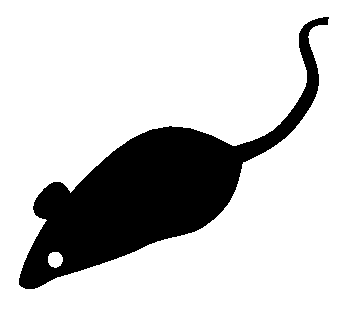
\includegraphics{aes2e-mouse.eps}
\caption{The spectral delay filter consists of \textit{M} allpass filters and an equalization filter.}
\end{figure}


\begin{figure*}
\centering
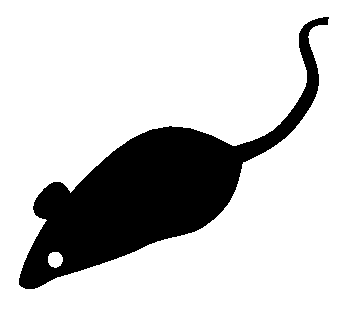
\includegraphics[width=23pc]{aes2e-mouse.eps}
\caption{This paper is organized as follows. In Section 1, we discuss the group delay of a cascade of first-order allpass filters and its relation to the chirp-like impulse response of the spectral delay filter. Furthermore, a multirate method to stretch the impulse response of the spectral delay filter is proposed. Section 2 discusses the amplitude envelope of the impulse response and suggests a design method for the equalizing filter. Section 3 presents application examples using the spectral delay filter. Section 4 concludes this paper.}
\end{figure*}
Filtering an audio signal with an allpass filter does not usually have a major effect on the signal's timbre. The allpass filter does not change the frequency content of the signal, but only introduces a phase shift or delay.
\begin{extract}
Filtering an audio signal with an allpass filter does not usually have
a major effect on the signal's timbre. The allpass filter does not
change the frequency content of the signal, but only introduces a
phase shift or delay. Audibility of the phase distortion caused by an
allpass filter in a sound reproduction system has been a topic of many
studies, see, e.g., \cite{DEK1}, \cite{DEK2}. In this paper, we
investigate audio effects \nobreak processing using high-order allpass filters that consist of many cascaded low-order allpass filters. These filters have long chirp-like impulse responses. When audio and music signals are processed with such a filter, remarkable changes are obtained that are similar to the spectral delay effect  \cite{DEK3}, \cite{DEK4}.
\end{extract}
Filtering an audio signal with an allpass filter does not usually have a major effect on the signal's timbre. The allpass filter does not change the frequency content of the signal, but only introduces a phase shift or delay. 
\[
\tau _\textrm{g} (\omega ) =  - \frac{{d\phi (\omega )}}{{d\omega }}.
\]
Audibility of the phase distortion caused by an allpass filter in a sound reproduction system has been a topic of many studies, see, e.g., \cite{DEK1}, \cite{DEK2}. In this paper, we investigate audio effects processing using high-order allpass filters that consist of many cascaded low-order allpass filters. These filters have long chirp-like impulse responses. When audio and music signals are processed with such a filter, remarkable changes are obtained that are similar to the spectral delay effect.
\begin{alphalist}
\item{}Green--function determined experimentally and published.
\item{}Black--function determined using similarity searches and published.
\item{}Red--function determined using similarity searches and determined in this study.
\item{}Blue--O-antigen structure unknown. Function determined using similarity searches and proposed in this study.
\end{alphalist}
Filtering an audio signal with an allpass filter does not usually have a major effect on the signal's timbre. The allpass filter does not change the frequency content of the signal, but only introduces a phase shift or delay. Audibility of the phase distortion caused by an allpass filter in a sound reproduction system has been a topic of many studies, see, e.g., \cite{DEK1}, \cite{DEK2}. 
%Enunciations
\begin{example}
In this paper, we investigate audio effects processing using high-order allpass filters that consist of many cascaded low-order allpass filters. These filters have long chirp-like impulse responses. 
\end{example}
Filtering an audio signal with an allpass filter does not usually have a major effect on the signal's timbre. The allpass filter does not change the frequency content of the signal, but only introduces a phase shift or delay. Audibility of the phase distortion caused by an allpass filter in a sound reproduction system has been a topic of many studies.
\begin{bulletlist}
\item{}Green--function determined experimentally and published.
\item{}Black--function determined using similarity searches and published.
\item{}Red--function determined using similarity searches and determined in this study.
\item{}Blue--O-antigen structure unknown. Function determined using similarity searches and proposed in this study.
\end{bulletlist}
Filtering an audio signal with an allpass filter does not usually have a major effect on the signal's timbre. The allpass filter does not change the frequency content of the signal, but only introduces a phase shift or delay. Audibility of the phase distortion caused by an allpass filter in a sound reproduction system has been a topic of many studies, see, e.g., \cite{DEK1}, \cite{DEK2}. In this paper, we investigate audio effects processing using high-order allpass filters that consist of many cascaded low-order allpass filters. These filters have long chirp-like impulse responses. When audio and music signals are processed with such a filter, remarkable changes are obtained that are similar to the spectral delay effect  \cite{DEK3}, \cite{DEK4}.
\begin{unnumlist}
\item{}Green--function determined experimentally and published.
\item{}Black--function determined using similarity searches and published.
\item{}Red--function determined using similarity searches and determined in this study.
\item{}Blue--O-antigen structure unknown. Function determined using similarity searches and proposed in this study.
\end{unnumlist}
Filtering an audio signal with an allpass filter does not usually have a major effect on the signal's timbre. The allpass filter does not change the frequency content of the signal, but only introduces a phase shift or delay. Audibility of the phase distortion caused by an allpass filter in a sound reproduction system has been a topic of many studies, see, e.g., \cite{DEK1}, \cite{DEK2}. In this paper, we investigate audio effects processing using high-order allpass filters that consist of many cascaded low-order allpass filters. These filters have long chirp-like impulse responses. When audio and music signals are processed with such a filter, remarkable changes are obtained that are similar to the spectral delay effect  \cite{DEK3}, \cite{DEK4}.

\section{SUMMARY}
Filtering an audio signal with an allpass filter does not usually have a major effect on the signal's timbre. The allpass filter does not change the frequency content of the signal, but only introduces a phase shift or delay. Audibility of the phase distortion caused by an allpass filter in a sound reproduction system has been a topic of many studies, see, e.g., \cite{DEK1}, \cite{DEK2}. In this paper, we investigate audio effects processing using high-order allpass filters that consist of many cascaded low-order allpass filters. These filters have long chirp-like impulse responses. When audio and music signals are processed with such a filter, remarkable changes are obtained that are similar to the spectral delay effect  \cite{DEK3}, \cite{DEK4}.

\section{CONCLUSION}
Filtering an audio signal with an allpass filter does not usually have a major effect on the signal's timbre. The allpass filter does not change the frequency content of the signal, but only introduces a phase shift or delay. Audibility of the phase distortion caused by an allpass filter in a sound reproduction system has been a topic of many studies, see, e.g., \cite{DEK1}, \cite{DEK2}. In this paper, we investigate audio effects processing using high-order allpass filters that consist of many cascaded low-order allpass filters. These filters have long chirp-like impulse responses. When audio and music signals are processed with such a filter, remarkable changes are obtained that are similar to the spectral delay effect  \cite{DEK3}, \cite{DEK4}. Note that articles might have a digital object identifier~\cite{DEK5}.

\section{ACKNOWLEDGMENT}
This research was conducted in fall 2008 when Vesa V\"alim\"aki was a visiting scholar at CCRMA, Stanford University. His visit was financed by the Academy of Finland (project no. 126310). The authors would like to Dr. Henri Penttinen for his comments and for the snare drum sample used in this work.

\bibliography{aes2e.bib}
\bibliographystyle{aes2e.bst}

% NOTE:
% - in case you are not using bibTex you have to manually edit the bibliograpy as below.
% - if submitting a bibTex file is not allowed you can copy the content from the aes2e.bbl file  
%\begin{thebibliography}{99}
%
%\newcommand{\enquote}[1]{``#1''}
%\providecommand{\url}[1]{\texttt{#1}}
%\providecommand{\urlprefix}{URL }
%\expandafter\ifx\csname urlstyle\endcsname\relax
%  \providecommand{\doi}[1]{[Online]. Available: \discretionary{}{}{}#1}\else
%  \providecommand{\doi}{doi:\discretionary{}{}{}\begingroup
%  \urlstyle{rm}\Url}\fi
%
%\bibitem{DEK1}
%D.~Preis, \enquote{Phase Distortion and Phase Equalization in Audio Signal
%  Processing---A Tutorial Review,} \emph{J. Audio Eng. Soc.}, vol.~30, no.~11,
%  pp. 774--779 (1982 Nov.).
%
%\bibitem{DEK2}
%J.~S. Abel, D.~P. Berners, \enquote{MUS424/EE367D: Signal Processing Techniques
%  for Digital Audio Effects,}  (2005), unpublished Course Notes, CCRMA,
%  Stanford University, Stanford, CA.
%
%\bibitem{DEK3}
%C.~Roads, \enquote{Musical Sound Transformation by Convolution,} presented at
%  the \emph{Int. Computer Music Conf.}, pp. 102--109 (1993).
%
%\bibitem{DEK4}
%C.~Roads, \emph{The Computer Music Tutorial} (MIT Press, Cambridge, MA), 1st
%  ed. (1996).
%
%\bibitem{DEK5}
%H.~Morgenstern, B.~Rafaely, \enquote{Spatial Reverberation and Dereverberation
%  Using an Acoustic Multiple-Input Multiple-Output System,} \emph{J. Audio Eng.
%  Soc}, vol.~65, no. 1/2, pp. 42--55 (2017 Jan.Feb.),
%  \doi{https://doi.org/10.17743/jaes.2016.0063}.
%  
%\end{thebibliography}

%Appendix
\appendix
\section*{APPENDIX}
Filtering an audio signal with an allpass filter does not usually have a major effect on the signal's timbre. The allpass filter does not change the frequency content of the signal, but only introduces a phase shift or delay. Audibility of the phase distortion caused by an allpass filter in a sound reproduction system has been a topic of many studies, see, e.g., \cite{DEK1}, \cite{DEK2}.
\begin{equation}
\phi (\omega ) =  - \omega  + 2\arctan \left( {\frac{{a_1 \sin \omega }}{{1 + a_1 \cos \omega }}} \right)
\end{equation}

In this paper, we investigate audio effects processing using high-order allpass filters that consist of many cascaded low-order allpass filters. These filters have long chirp-like impulse responses. When audio and music signals are processed with such a filter, remarkable changes are obtained that are similar to the spectral delay effect  \cite{DEK3}, \cite{DEK4}.


\begin{nomenclature}[PAMPs]
\subsection*{NOMENCLATURE}
\nomentry{a$_c$}{condensation coefficient condensation coefficient condensation coefficient}


\nomentry{TLR}{Toll-like receptor}

\nomentry{PAMPs}{pathogen-associated molecular patterns condensation coefficient condensation}
\end{nomenclature}

%Biography
 \biography{A1firstname A1lastname}{a.eps}{A1firstname A1lastname is professor of audio signal processing at Helsinki University of Technology (TKK), Espoo, Finland. He received his Master of Science in Technology, Licentiate of Science in Technology, and Doctor of Science in Technology degrees in electrical engineering from TKK in 1992, 1994, and 1995, respectively. His doctoral dissertation dealt with fractional delay filters and physical modeling of musical wind instruments. Since 1990, he has worked mostly at TKK with the exception of a few periods. In 1996 he spent six months as a postdoctoral research fellow at the University of Westminster, London, UK. In 2001-2002 he was professor of signal processing at the Pori School of Technology and Economics, Tampere University of Technology, Pori, Finland. During the academic year 2008-2009 he has been on sabbatical and has spent several months as a visiting scholar at the Center for Computer Research in Music and Acoustics (CCRMA), Stanford University, Stanford, CA. His research interests include musical signal processing, digital filter design, and acoustics of musical instruments. Prof. V\"alim\"aki is a senior member of the IEEE Signal Processing Society and is a member of the AES, the Acoustical Society of Finland, and the Finnish Musicological Society. He was the chairman of the 11th International Conference on Digital Audio Effects (DAFx-08), which was held in Espoo, Finland, in 2008.}
 \biography{A2firstname A2lastname}{b.eps}{A2firstname A2lastname is a consulting professor at the Center for Computer Research in Music and Acoustics (CCRMA) in the Music Department at Stanford University where his research interests include audio and music applications of signal and array processing, parameter estimation, and acoustics. From 1999 to 2007, Abel was a co-founder and chief technology officer of the Grammy Award-winning Universal Audio, Inc. He was a researcher at NASA/Ames Research Center, exploring topics in room acoustics and spatial hearing on a grant through the San Jose State University Foundation. Abel was also chief scientist of Crystal River Engineering, Inc., where he developed their positional audio technology, and a lecturer in the Department of Electrical Engineering at Yale University. As an industry consultant, Abel has worked with Apple, FDNY, LSI Logic, NRL, SAIC and Sennheiser, on projects in professional audio, GPS, medical imaging, passive sonar and fire department resource allocation. He holds Ph.D. and M.S. degrees from Stanford University, and an S.B. from MIT, all in electrical engineering. Abel is a Fellow of the Audio Engineering Society.}
\end{document}
